\section{Generative Adversarial Networks}
GAN (Generative Adversarial Networks), Ian Goodfellow ve Montreal Üniversitesi'nden diğer araştırmacılar tarafından 2014 yılında tanıtılmıştır. Üretken yapay zeka kümesine ait bir sinir ağıdır. İki sinir ağından oluşmaktadır. Generator (Üretici) ve Discriminator (Ayırıcı). Birbirlerine karşı yerleştirilirler. Generator, yeni örnekleri oluşturur. Discriminator, oluşturulan örneklerin gerçekliğini değerlendirir. Generator tarafından üretilen verileri gerçek ve sahte olarak sınıflandıran ikili bir sınıflandırıcıdır. Eğitim verileri buraya yüklenir. 

GAN'ın avantajları;
\begin{itemize}
	\item Gerçekçi Veri Üretimi
	\item Çeşitli Veri Üretimi
	\item Denetimsiz Öğrenme
	\item Görüntüden Görüntüye Çeviri
	\item Yaratıcı Uygulamalar
\end{itemize}

GAN'ın dezavantajları;
\begin{itemize}
	\item Eğitim İstikrarsızlığı
	\item Mod Daraltma
	\item Değerlendirme Metrikleri
	\item Hiperparametre Hassasiyeti
	\item Hesaplamalı Kaynaklar
\end{itemize}

Bazı GAN türleri:

\begin{enumerate}
    \item DCGAN (Deep Convolutional GAN)
    \item WGAN (Wasserstein GAN)
    \item SRGAN (Super Resolution GAN)
    \item pix2pix (Image to Image)
    \item CycleGAN (Cycle Generative)
    \item StackGAN (Stacked GAN)
    \item ProGAN (Progressive Growing)
    \item StyleGAN (Style-Based GAN)
    \item VQGAN (Vector Quantized)
    \item SGAN
    \item SAGAN
    \item AC-GAN
    \item GauGAN
    \item GFP-GAN
\end{enumerate}

\subsection{Çalışma Adımları}
Üretici rastgele gürültüden gelen bir girişi kullanarak veri setine benzeyen yeni örnekler üretir. Ayırıcı, bu örnekleri gerçek veya sahte olarak sınıflandırır. İki ağ da birbirine karşıdır. Üretici, ayırıcının sahte veri örneklerini gerçek olarak sınıflandırmasını engellemeye çalışırken, ayırıcı gerçek ve sahte örnekleri daha doğru bir şekilde ayırt etmeye çalışır. Bu sürekli rekabet ve geri besleme döngüsü sonucunda, hem üretici ağ daha gerçekçi veri örnekleri üretmeyi öğrenirken hem de ayırt edici ağ daha hassas bir şekilde gerçek ve sahte örnekleri ayırt etmeyi öğrenir.

Eğitim sırasında üretici ve ayırt edici ağ arasında bir denge sağlanmalıdır. Eğer üretici ağ çok iyi olursa ve ayırt edici ağ sahte verilerle gerçek verileri ayırt edemez hale gelirse model başarısız olabilir. 

\begin{figure}[h]
    \centering
    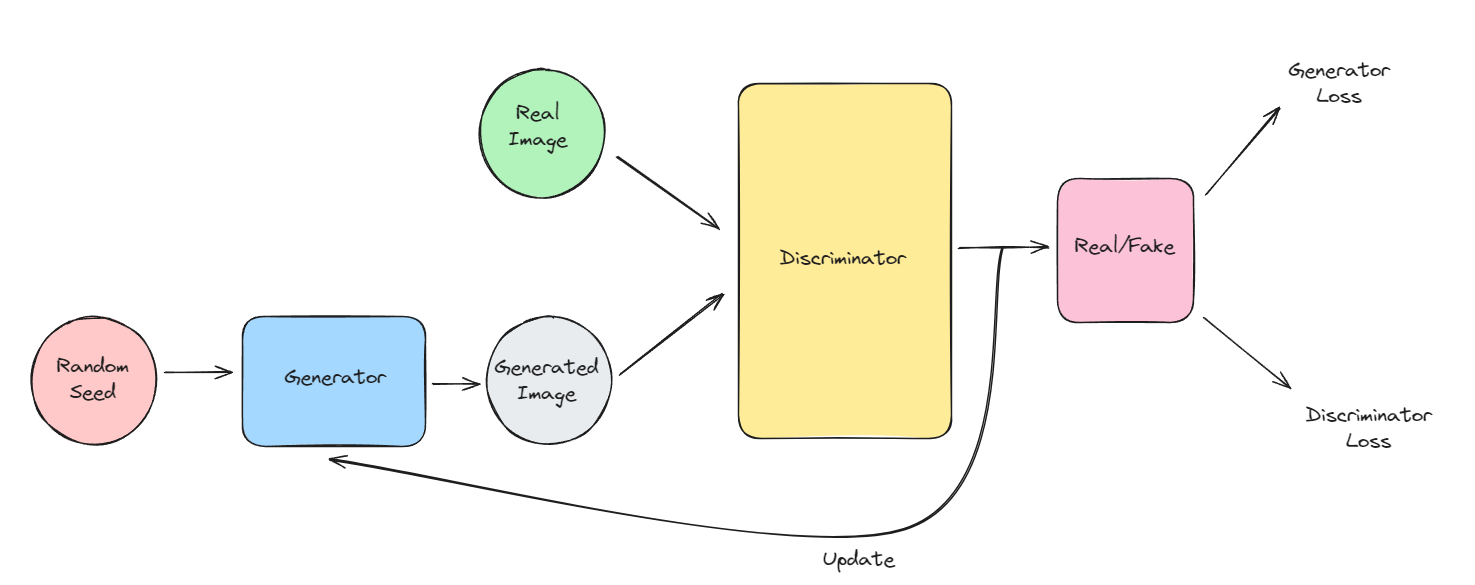
\includegraphics[width=1\textwidth]{images/gan_architecture.png}
    \caption{GAN mimarisi.}
    \label{fig:enter-label}
\end{figure}

\subsection{Deep Convolutional GAN (DCGAN)}
2015 yılında Radford ve diğerleri tarafından yayınlanmıştır. GAN'dan farkı FC (tam bağlantılı) katmanlar yerine CNN kullanır. DCGAN, özellikle resimlerin üretilmesi üzerine odaklanmış olduğu için CNN mimarisini kullanır. CNN'ler genelde görüntüde korelasyon ararlar bu da DCGAN'ın resim ve videolar için daha uygun olduğu anlamına gelir. Kayıp fonksiyonu olarak "Binary Cross-entropy" kullanır.

\subsection{Wasserstein GAN (WGAN)}
2017 yılında Arjovsky ve diğerleri tarafından tanıtılmıştır. Eğitimin kararlılığını artırmak için Wasserstein Distance (Wasserstein Mesafesi) kullanır. Bu daha kararlı ve düzgün bir gradyan akışı sağlar.  Wasserstein mesafesi, iki dağılım arasındaki en küçük taşıma maliyetini ölçer. Bu, bir dağılımı diğerine dönüştürmek için gereken minimum ortalama maliyeti ifade eder. Taşıma maliyeti, her bir parçacığın bir noktadan diğerine taşınması için gereken ortalama maliyettir. Wasserstein mesafesi, üretilen görüntülerin gerçek veri dağılımına ne kadar yakın olduğunu ölçer. Mode Collapse (mod çakışması) ve vanishing gradients (kaybolan gradyanlar) problemini çözmüştür. Mod çakışması, generator modelin çıktısının gerçek veri dağılımının yalnızca belirli bir alt kümesini yansıtmasıdır. Generator ağın her yinelemesinde discriminator ağın belirli bir alt kümeye aşırı uyum sağlaması sonucu oluşur. Kaybolan gradyanlarda ise Discriminator ağ, generator modelin ürettiği örnekleri kolayca ayırt edebilirse, generator model daha güvenli örnekler üretmeyi tercih edebilir. Bu da çeşitlilik eksikliğine neden olur.

\subsubsection{Lipschitz Constraint}
WGAN formülasyonunda, modelin üretimindeki kararlılığın artırılması için discriminator ağın Lipschitz sürekli olduğunu garanti eden bir kısıtlama getirilmiştir. Lipschitz sürekliliği bir fonksiyonunun davranışının istikrarlı ve tahmin edilebilir olmasını sağlar. Bir fonksiyon, Lipschitz sürekliliğini sağlıyorsa, bu fonksiyonun davranışı belirli bir ölçüde "düzenli" olarak kabul edilir. Ancak, WGAN'da bu kısıtlamanın uygulaması zor olabilir. Hiperparametre "C" doğru ayarlanmadığında model düşük kaliteli görüntüler üretebilir.

\subsection{Wasserstein GAN with Gradient Penalty (WGAN-GP)}
Gulrajani ve arkadaşları tarafından tanıtılmıştır. Eğitim sırasında Lipschitz kısıtlamasını elde etmek için Gradient Penalty (Gradyan Cezası) yöntemini kullanmasıdır. Gradient Penalty, discriminator ağı eğitiminde Lipschitz sürekliliğini zorlamak için ek bir terim olarak kullanılır. Gradient Penalty, discriminator ağın gradientlerinin normunu cezalandırarak çalışır. Bu, discriminator ağın gradyanlarının belirli bir sınıra yakın olmasını ve böylece Lipschitz sürekliliğini sağlamasını sağlar.

\subsection{Conditional GAN (cGAN)}
Generator modelin belirli bir koşula göre (bir sınıf etiketi) öğrenilmesini sağlar. cGAN'da discriminator ağ, gerçek ve üretilen görüntü arasındaki farkı belirlerken bir koşul vektörünü ele alır ve bu vektörü göz önünde bulundurarak sınıflandırma yapar. Normal bir GAN modelinde gizli vektör eşlemesinin görüntünün gerçek özellikleriyle nasıl ilişkili olduğunu bilmiyoruz, bu nedenle bir "kara kutu" gibidir. Belirli sonuçlar elde etmek için bu özellikleri manipüle edemeyiz. Görüntü rastgele bir gürültüden oluşur. cGAN bu sorunu giderir.

\subsection{Pix-to-Pix}
cGAN'ın bir türevidir. Bir görüntüden diğerine çeviri yapmak için kullanılır. Bir giriş görüntüsü alır ve bu giriş görüntüsünü belirli bir çıktı formatına çevirir. 

\subsection{Cycle-Consistent GAN (CycleGAN)}
Bi görüntüden diğerine çeviri yapmak için kullanılır. Pix-to-pix gibi doğrudan eşleştirilmiş eğitim verilerine ihtiyaç duymaz. Bunun yerine "unsupervised learning (denetimsiz öğrenme)" prensibini kullanır. Cycle Consistency Loss, dönüşüm yapılırken orijinal görüntünün yeniden oluşturulmasını zorunlu kılar. Yani bir görüntü bir dönüşüme uğradıktan sonra tekrar orijinal hale geldiğinde, başlangıç ve sonuç arasında bir tutarlılık sağlar. Pix-to-pix'e kıyasla daha maliyetli ve zaman alıcı bir eğitim sunar. Renk ve doku değişikliklerini içeren çeviri görevlerinde yöntem genellikle başarılıdır. Örneğin at-zebra, elma-portakal dönüşümü.

\subsection{Super Resolution GAN (SRGAN)}
2017 yılında Ledig ve diğerleri tarafından yayınlanmıştır. Düşük çözünürlüklü (Low-Resolution - LR) giriş görüntülerini yüksek çözünürlüklü (High-Resolution - HR) görüntülere dönüştürmeyi amaçlar. Generator, düşük çözünürlüklü giriş görüntüsünü alır ve bunu yüksek çözünürlüklü bir çıktıya dönüştürmeye çalışır. Sub-pixel convolution kullanır. Sub-pixel convolution, giriş görüntüsünü daha yüksek boyuta genişletmek yerine, gizli katmanlarda işlenirken yüksek boyutlu bir tensör oluşturur. Daha sonra bu tensör, bir kanal grubunu, pikselleri birleştirerek daha büyük bir tensör oluşturmak için yeniden boyutlandırır.

\subsection{Enhanched Super Resolution GAN (ESRGAN)}
2018 yılında X. Wang ve diğerleri tarafından tanıtılmıştır. SRGAN'ın geliştirilmiş bir versiyonudur. ESRGAN'da, perceptual loss, content loss gibi özel kayıp fonksiyonları kullanılabilir. Bu kayıp fonksiyonları, üretilen görüntülerin daha fazla detay ve daha gerçekçi olmasını sağlamak için kullanılır. ESRGAN, transfer learning kullanarak önceden eğitilmiş bir VGG19 modelinin özelliklerini kullanabilir. Bu, generator ağın daha iyi sonuçlar elde etmek için daha fazla bilgiye erişmesini sağlar.

\subsection{Progressive Growing of GAN (ProGAN)}
2017 yılında NVIDIA tarafından tanıtılmıştır. GAN'ların eğitimini aşamalı olarak gerçekleştiren ve daha yüksek çözünürlüklü görüntülerin üretimesini sağlayan bir modeldir. Düşük çözünürlüklü görüntülerden başlayarak yavaş yavaş daha yüksek çözünürlüklü görüntülere geçiş yapar. İlk olarak, generator ağ düşük çözünürlüklü görüntüleri üretmek için eğitilir. Her aşamada, generator ve discriminator ağ daha fazla katman ekler. Transfer learning yöntemlerini kullanarak önceki aşamalarda öğrenilen bilgileri daha sonraki aşamalara aktarır.

\subsection{StyleGAN}
2018 yılında NVIDIA tarafından tanıtılmıştır. Yüksek kaliteli ve yüksek çözünürlüklü insan yüzü ve diğer görsel içeriklerin üretilmesi için kullanılır.

\subsection{Vector Quantized GAN (VQGAN)}
Görsel verilerin temsillerini kodlamak ve yeniden oluşturmak için kullanılır. Giriş olarak verilen görsel veri üzerinde CNN kullanarak özellik çıkarımı yapılır. Elde edilen özellikler vektör kuantizasyonundan geçilir. Vektör kuantizasyonu, özellik vektörünü sabit bir sayıda semantik olarak anlamlı kümelerden birine atar. Bu, özellik vektörünün boyutunu azaltır ve daha basit bir temsil elde edilmesini sağlar. Kuantize edilmiş vektör, bir kodlayıcı kullanılarak daha düşük boyutlu bir vektöre kodlanır. Bu, görüntünün daha düşük boyutlu bir temsilini oluşturur. Kodlanmış vektör, bir dekoder kullanılarak yeniden oluşturulur. Bu, orijinal görüntünün yeniden oluşturulmasını sağlar. 

\subsection{GauGAN}
NVIDIA tarafından geliştirilmiştir. Görüntülerin segmentasyonunu ve sentezini geliştirmek için kullanılır. Temel fikri, basit bir çizimle başlayarak karmaşık ve gerçekçi görüntüler oluşturmaktır. Kullanıcı, bir çizim arayüzü üzerinden basit bir çizim oluşturur. Çizim, farklı renklerle ve şekillerle temsil edilen nesneleri içerir. GauGAN, kullanıcının çizimini alır ve farklı nesneleri otomatik olarak tanımlar ve segmente eder. Bu, çizimin her bölgesinin hangi nesneye ait olduğunu belirlemek için bir segmentasyon aşamasını içerir. GauGAN, her bir nesne için bir özellik haritası oluşturur. Bu özellik haritaları, her bir nesnenin geometrik şeklini, renklerini ve diğer özelliklerini temsil eder. Her bir özellik haritası, o nesnenin piksel düzeyinde ayrıntılı bir temsilini içerir. GauGAN, özellik haritalarını birleştirir ve gerçekçi bir görüntü oluşturur.

\subsection{Generative Face Completion (GFP-GAN)}
Yüz görüntülerinin tamamlanması ve restore edilmesi için kullanılır. Yarı eksik veya bozulmuş bir yüz görüntüsünü alır. Eksik yüz görüntüsünü bir latent uzayda kodlamak için bir kodlayıcı kullanır. Bu, eksik görüntünün temsilini elde etmek ve işlemek için bir vektör oluşturur. Kodlanmış eksik görüntü vektörü bir dekoder kullanarak tamamlanır. 

\subsection{Auxiliary Classifier GAN (ACGAN)}
Standart GAN mimarisine ek olarak 1 adet sınıflandırıcı eklenmiştir. Bu sınıflandırıcı, üretilen verinin hangi sınıfa ait olduğunu tahmin etmeye çalışır. Böylece, üretilen verinin hem gerçekçi olması hem de belli bir sınıfa ait olması sağlanır.

\begin{itemize}
    \item \textbf{Adversarial Loss}: Üretilen örneğin gerçek mi sahte mi olduğunu ölçer.
    \item \textbf{Auxiliary Loss}: Üretilen örneğin hangi sınıfa ait olduğunu ölçer.
\end{itemize}

\subsection{Boundary Equilibrium GAN (BEGAN)}

BEGAN, bir denge noktası (equilibrium point) ile generator ve discriminator arasındaki dengeyi kurar. Böylece, modelin overfitting ve mode collapse gibi sorunlarla karşılaşma olasılığı azalır. 

\begin{enumerate}
    \item Eğitime başlarken, denge parametresi küçük bir değere ayarlanır. 
    \item Ayırıcının yaptığı hata kullanılarak, denge parametresi güncellenir. Eğer ayırt edici çok fazla hata yapıyorsa, denge parametresi artıralarak üreticiye daha fazla özgürlük verir. Eğer ayırt edici çok az hata yapıyorsa, denge parametresi azaltılarak üretici daha kısıtlanır.
\end{enumerate}

\subsection{Boundary-Seeking GAN (BSGAN)}

BSGAN'ın temel farkı, ayrımcının kararlarının olasılık dağılımının sınırlarında toplanmasını sağlamasıdır. Bu, eğitim sırasında üretilen verinin kalitesini artırmakta ve daha stabil bir eğitim süreci sunmaktadır.

\begin{enumerate}
    \item Rastgele gürültüden görüntüler üretilir.
    \item Ayırıcı, üretilen örneklerin gerçek olup olmadığını belirlerken aynı zamanda bu örneklerin veri dağılımındaki konumunu da değerlendirir.
    \item Ayırıcı, üretilen örneklerin veri dağılımının sınırlarına daha yakın olduğunu tespit ederse, üretiyici bu yönde teşvik eder.
    \item Üretici ve ayırt edici arasındaki bu etkileşim, bir denge içinde sürdürülür.
\end{enumerate}

\subsection{Cluster GAN (Clustering-aware GAN)}

Kümeleme ve jeneratif modellemeyi birleştirir. Cluster GAN, hem gerçek verilerin dağılımını öğrenmek hem de veriyi kümelere ayırmak amacıyla tasarlanmıştır. Gerçek verilerin altında yatan gizli yapıları öğrenirken, üretilen veriyi bu yapılara göre kategorize ederek yüksek kalitede örnekler oluşturmayı hedefler. İçerisinde Generator ve Discriminator'a ek olarka bir adet Encoder bulunur. Bu encoder, gerçek veriyi gizli uzaya kodlayarak, bu verilerin nasıl dağıldığını öğrenir.

\begin{enumerate}
    \item Rastgele gürültüden görüntüler üretilir.
    \item Kümeleme modülü, üretilen örnekleri belirli sayıda kümeye ayırır.
    \item Kümeleme sonuçları, hem üreticiye hem de ayırt ediciye geri beslenir. Üretici, örneklerini daha iyi tanımlanmış kümelere üretmeye çalışırken, ayırt edici de bu kümeleri ayırt etmeye çalışır.
\end{enumerate}

\subsection{Context-Conditional GAN (CCGAN)}

Modelin veri üretim sürecinde belirli bir bağlamı (context) dikkate almasını sağlar. Bu model, belirli bir koşula göre veri üretebilir. Bağlam, modelin veri üretiminde dikkat etmesi gereken koşullu bilgiyi sağlar. Bu, metin, sınıf etiketi, görüntü özelliği gibi herhangi bir bağlamsal bilgi olabilir. Üretici, girdiye yalnızca rastgele bir gürültü vektörü değil, aynı zamanda belirli bir bağlamda koşullu bilgi de alır. Üretici, bu bilgiyi dikkate alarak koşula uygun veri üretir. 

\subsection{Context-Encoder GAN (CEGAN)}

Eksik veya kısmı verileri tamamlama (inpainting) problemlerinde kullanılan bir GAN çeşididir. Eksik bir girdiyi kullanarak bu eksikliği doldurmak ve orijinal tam veri ile uyumlu bir çıktı üretmek üzere tasarlanmıştır. Özellikle gürültü tamamlama, ses veya diğer veri türlerinin eksik kısımlarının yeniden oluşturulmasında etkilidir. Bağlamsal bilgiyi dikkate alarak eksik veriyi tahmin etmeye çalışır.

\subsection{Coupled GAN (CoGAN)}

İki farklı ama ilgili veri dağılımını öğrenmek ve bu iki dağılımı eşleştirmek amacıyla kullanılan bir GAN türüdür. CoGAN, iki farklı veri kümesinden benzer yapılsal özelliklere sahip veriler üretmek için tasarlanmıştır. Bu yöntem, iki GAN'ın ağırlık paylaşımı yoluyla birbirleriyle senkronize çalışmasıyla, çiftler halinde uyumlu veri üretimi sağlar. Bu GAN'lar birbirinden bağımsız çalışsa da, belirli katmanlar arasında ağırlık paylaşımı yaparak iki veri kümesi arasındaki ortak özellikleri öğrenirler. Bu mimaride, her iki GAN'ın üretici ve ayrımcıları bulunur, ancak belirli katmanlar ortak kullanılır. 

\subsection{Disco GAN}

İki farklı veri kümesi arasındaki ilişkili fakat farklı özellikleri öğrenmeye ve dönüştürmeye odaklanan bir GAN türüdür. İki farklı alan arasında birbiriyle uyumlu veriler üreterek, iki veri kümesi arasında çift yönlü dönüştürme yapmayı hedefler. Örneğin, bir alandaki veriyi diğer alana dönüştürme ve ardından bu dönüşümü tekrar orijinal alana geri döndürme işlemini gerçekleştirir. Disco GAN, çembersel bir kayıp fonksiyonu kullanır. Bu sayede, bir veri önce bir domaine dönüştürülüp sonra tekrar ilk domainine geri döndürüldüğünde, başlangıçtaki veriye mümkün olduğunca yakın bir sonuç elde edilmesi hedeflenir.

\subsection{Deep Regret Analytic GAN (DRAGAN)}

Temel amacı, GAN'larda karşılaşılan eğitim dengesizliklerini ve başarısızlıkları engellemektedir. Bu dengesizlikler genellikle ayrıştırıcı ağın çok hızlı bir şekilde güçlenmesi ve üretici ağın iyi öğrenememesi durumlarında ortaya çıkar. DRAGAN, bu sorunu çözmek için ayrıştırıcıya, eğitim sırasında ek regülarizasyon teknikleri uygular.  Gradient Regularization (Gradient Penalty) sayesinde ayrıştırıcının eğitimi sırasında hatalı veya aşırı güçlü öğrenmesi engellenir. Böylece, ayrıştırıcı çok hızlı şekilde öğrenip üreticiyi başarısız kılacak kadar güçlü hale gelmez. 

\subsection{DualGAN}

iki yönlü görntü dönüşümleri için kullanılır. Çift yönlü dönüşümler, bir görüntü alanından diğerine ve ardından tekrar geri dönüşümü mümkün kılmayı hedefler. Örneğin siyah-beyaz bir görüntüyü renklendirmek ve ardından bu renklendirilmiş görüntüyü tekrar siyah-beyaz hale getirmek gibi görevlerde kullanılır. Cycle Consistency Loss, iki veri alanı arasındaki dönüşümlerin mantıklı olmasını sağlar. Dönüştürülmüş veri, tekrar orijinal veri alanına geri çevrilir. Örneğin $X \rightarrow Y \rightarrow X$ dönüşümü, başlangıçtaki X görüntüsüne mümkün olduğunca yakın olmalıdır. Bu, "cycle consistency loss" ile ölçülür.

\subsection{Energy-based GAN (EBGAN)}

EBGAN, klasik GAN yapısını enerji temelli bir yaklaşımla yeniden formüle eden bir modeldir. Ayrıştırıcıyı bir enerji fonksiyonu olarak ele alır ve bu fonksiyonun çıktısının, bir veri örneğinin gerçek veya sahte olupğ olmadığını belirlediği bir enerji temelli model ortaya koyar. Ayrıştırıcı, bu enerji seviyesini minimize etmeye odaklanır. Gerçek veriler için enerji seviyesini düşürmeye çalışırken, sahte veriler için bu seviyeyi artırır. Ayrıştırıcının çıktısı, bir veri örneğinin "enerjisini" temsil eder. Bu enerji bir reconstruction loss (yeniden yapılandırma hatası) olarak yorumlanır. Gerçek verilerde bu hata daha düşük, sahte verilerde ise daha yüksek olacak şekilde optimize edilir.

\subsection{Information Maximizing GAN (InfoGAN)}

Denetimsiz öğrenme ile anlamlı ve yorumlanabilir veri temsilleri elde etmeye odaklanır. InfoGAN, üretilen veriler üzerinde kontrol sahibi olmayı sağlar ve gizli değişkenlerin bazılarını anlamlı hale getirir. Bu, üretilen örneklerdeki belirli faktörlerin manipüle edilmesini mümkün kılar. Ayrıştırıcı, sahte veya gerçek verileri ayırt ederken aynı zamanda üreticinin ürettiği bilgiyi yeniden yapılandırmaya çalışır. Bu yeniden yapılandırma işlemi ile bilgi kaybı (mutual information) minimize edilir. Q ağı, ayrıştırıcı ile birlikte çalışarak bilgi vektörünün geri kazanılmasını sağlar. Verilen sahte örneklere göre bilgi vektörünü tahmin eder. 

\subsection{Least Squares GAN (LSGAN)}

LSGAN'da ayrıştırıcıda kullanılan kayıp fonksiyonu binary cross entropy yerine ortalama kare hata (mean squared error) olarak değiştirilmiştir. Gerçek veriler için yüksek değerler, sahte veriler için düşük değerler üretir. LSGAN'da ayrımcının çıktısı gerçeklik ve sahtelik arasındaki farkı ifade eder ve bu fark ortalama kare ile hesaplanır. Gerçek veriler için hedef değer 1, sahte veriler için hedef değer 0'dır. Ayrıştırıcının kaybı, gerçek ve sahte verilerin tahmin edilen değerleri ile bu hedef değerler arasındaki ortalama kare hatadır. Üreticinin amacı sahte veriler için tahmin ettiği değerlerin 1'e ne kadar yakın olduğunu sağlamak için kaybını minimize eder. Bu, üreticinin ayrıştırıcıyı daha iyi yanıltmasını sağlar.

\subsection{Unified GAN for Image-to-Image Translation (UNIT)}

Birden fazla görüntü dönüşüm görevini tek bir modelle gerçekleştirebilen bir modeldir. Encoder, giriş görüntüsünü özellik haritalarına dönüştüren bir ağdır. Decoder, özellik haritalarını hedef alanda uygun bir görüntüye dönüştürür. Domain-Agnostic Encoder, hem kaynak hem de hedef alanlar için ortak bir encoder kullanılır. Bu, modelin genel özellikleri öğrenmesini sağlar. Domain-Specific Encoder, her bir alan için özel decoder kullanılır. Bu, her alanın özgüllüklerini yakalamak için gereklidir. Domain Classifier, üretilen görüntülerin hangi alana ait olduğunu tahmin eden bir bileşendir. Bu, alanlar arasındaki farklılıkları öğrenmeye yardımcı olur. 

\subsection{Multimodal Unsupervised Image-to-Image Translation (MUNIT)}

Çok modlu ve denetimsiz görüntü şekil çevirisi için geliştirilmiş bir generatif modeldir. MUNIT, bir görüntünün stilini ve içeriğini ayırarak, çeşitli stiller arasında dönüşüm yapabilen ve çeşitli içeriklerle uyumlu olan bir model sunar. İçerik kodlayıcı (content encoder), girdi görüntüsünün içeriğini çıkarır ve içerik özelliklerini temsil eden bir vektör üretir. Stil kodlayıcı (style encoder), girdi görüntüsünün stil özelliklerini çıkarır ve stil özelliklerini temsil eden bir vektör üretir.

\begin{enumerate}
    \item Girdi görüntüsü, içerik ve stil kodlayıcıları tarafından işlenir. İçerik kodlayıcı görüntünün içeriğini temsil eden bir vektör oluştururken, stil kodlayıcı, stil özelliklerini temsil eden bir vektör oluşturur.
    \item İçerik vektörü ve stil vektörü, dönüşüm ağına (generator) beslenir. Dönüşüm ağı, bu bilgileri birleştirerek hedef stilde dönüştürülmüş bir görüntü üretir.
    \item Üretilen görüntüler, ayrıştırıcı tarafından değerlendirilir. Ayrıştırıcı, görüntülerin gerçekliği ve içerik-stil uyumu hakkında geri bildirim sağlar.
    \item İçerik kaybı, üretilen görüntünün içerik vektörünü kaynak içerik vektörü ile karşılaştırarak hesaplanır. Stil kaybı, üretilen görüntünün stil vektörünü hedef stil vektörü ile karşılaştırarak hesaplanır. Adversarial (gerçek-sahte) kayıp, ayrıştırıcı tarafından hesaplanan görüntülerin gerçekliğini değerlendirir.
    \item Hesaplanan hatalar kullanılarak üretici ve ayrıştırıcı ağları güncellenir.
\end{enumerate}

\subsection{Pixel-wise Domain Adaption (PixelDA)}

Bir görüntü setinin başka bir kaynaktan başka bir kaynağa dönüştürülmesi gereken durumlarda kullanılır. Özellik çıkarıcı (feature extractor) ve uyum ağı (adaptation) networkten oluşur. Özellik çıkarıcı (feature extractor), görüntüleri işleyerek anlamlı özellikler çıkarır. Her iki alanda da (kaynak ve hedef) ortak bir temsil öğrenir. Uyum ağı (adaptation network), özellikleri her iki alan arasında uyumlu hale getirmek için çalışır. Bu ağ, kaynak ve hedef alanlardaki özelliklerin uyumlu olmasını sağlar. Bu iki alan arasındaki farklılıkları minimize etmeye çalışır.  Reconstruction Loss (Geri Dönüşüm Kaybı), özelliklerin doğru bir şekilde uyum sağladığını kontrol etmek için kullanılır. Bu kayıp, dönüştürülmüş görüntülerin kaynaktan hedef alana doğru bir şekilde haritalanıp haritalanmadığını kontrol eder. 

\begin{enumerate}
    \item Kaynak ve hedef görüntüler, özellik çıkarıcı tarafından işlenir. Bu, her iki alanda da ortak bir özellik temsilinin elde edilmesini sağlar.
    \item Özellikler, uyum ağı tarafından dönüştürülür. Bu, kaynak ve hedef alanlar arasındaki farklılıkları azaltmak için yapılır. Özelliklerin uyumlu hale gelmesi sağlanır.
    \item Dönüştürülmüş özellikler, kaynak görüntülerin hedef görüntülere dönüşümünü sağlar. Geri dönüşüm kaybı hesaplanır ve uyum ağı bu kaybı minimize etmek için eğitilir.
    \item Özelliklerin doğru şekilde çıkarıldığını ve sınıflandırıldığını kontrol eden bir sınıflandırma ağı kullanılır. Bu, modelin hedef alan üzerinde doğru sınıflandırmalar yapabilmesini sağlar.
    \item Özellik çıkarıcı, uyum ağı ve sınıflandırma ağı, geri dönüşüm ve sınıflandırma kayıplarına göre güncellenir.
\end{enumerate}

\subsection{Relativistic GAN}

Relativistic GAN, gerçek ve sahte görüntüleri tek tek değerlendirmek yerine, bunları birbiriyle karşılaştırır. Bu yaklaşım, ayrıştırıcının daha iyi bir göreceli değerlendirme yapmasını sağlar. Relativistic Loss, ayrıştırıcının gerçek ve sahte görüntüler arasındaki göreceli farklı öğrenmesini sağlar.

\subsection{Semi-Supervised GAN}

GAN içinde yarı denetimli öğrenmeyi kullanan bir modeldir. Bu model, etiketlenmiş ve etiketlenmemiş verilerle öğrenme sürecini destekler. SSGAN'de ayrımcı ağı ayrıca sınıflandırma görevini de yerine getirir. Bu, ayrımcının her görüntüyü hem gerçek/sahte hem de sınıf bilgisi açısından değerlendirmesini sağlar.

\subsection{Softmax GAN}

GAN içinde Softmax fonksiyonunu kullanarak, özellikle sınıflandırma problemlerini çözme ve yüksek kaliteli veri üretme konusunda geliştirilmiş bir modeldir. Softmax GAN, klasik GAN mimarisine ek olarak Softmax fonksiyonunu kullanarak sınıflandırma işlevselliği ekler. Softmax Katmanı, Ayrımcı ağına entegre edilir ve verilerin farklı sınıflara ait olma olasılıklarını hesaplar. Softmax fonksiyonu, bir dizi olasılığı normalize ederek, her bir sınıf için olasılıkları toplar ve bu olasılıkların toplamı 1 olur. Ayrımcı ağı, gerçek ve sahte verilerden özellikler çıkarır. Bu özellikler, Softmax katmanı tarafından sınıflandırma yapılacak şekilde işlenir. Generator ve ayrımcı ağları, Softmax fonksiyonunun hesapladığı sınıf kaybı ve gerçek/sahte kayıplarına göre güncellenir.

\subsection{Star GAN}

Çeşitli veri kümeleri üzerinde çoklu alanlarda (domain) verileri dönüştürmek için kullanılan bir modelidir. StarGAN, tek bir model kullanarak farklı alanlarda veri dönüştürme işlemlerini gerçekleştirebilir. Domain Classifier (Alan Sınıflayıcı), üretici ve ayrımcıdan bağımsız olarak çalışır ve verilerin hangi alana ait olduğunu tahmin eder. 

\newpage